\section{Background}

%%%%%%%%%%%%%%%%%%%%%%%%%%%%%%%%%%%%%%%%%%%%%%%%%%%%%%%%%%%%%%%%%%%%%%%%%%%%%%
\subsection{Runtime Scheduling}

\begin{slide}
    \begin{itemize}
        \item<1-> Schedulers can be defined in a discrete manner:
            \begin{enumerate}
                \item {\em Choose} a process from set,
                \item {\em Reduce} it,
                \item {\em Update} private scheduler state.
            \end{enumerate}
        \item<2-> Statistics can be gathered at every step about process:
            \begin{itemize}
                \item Timestamp of last run,
                \item Number of reductions, \etc
            \end{itemize}
        \item<3-> {\sl What statistics are useful?}
    \end{itemize}
    \inote{
        \item<2-> We can look at process schedulers like a function:
            \begin{itemize}{\scriptsize
                \item Takes a set of processes, and some private state.
                \item Job of the function is to choose a process, and run it for a bit.
                \item Then, based on what happened while running process, we update the state.
              }
            \end{itemize}
        \item<2-> Big questions: How are we choosing a process? What should effect our decision?
        \item<3-> Timestamp of last run? $\rightarrow$ 
            \begin{itemize}{\scriptsize 
                \item Choose always most recent, it's a batch scheduler.
                \item Choose oldest, we get something called Round-Robin.
                }
            \end{itemize}
        \item<3-> Number of reductions? $\rightarrow$ longevity = might want to 
                                                        give someone else a go.
        \item<3-> What are useful, and what do they tell us about the state of 
                the system? Well this leads us to cooperativity.
    }
\end{slide}


%%%%%%%%%%%%%%%%%%%%%%%%%%%%%%%%%%%%%%%%%%%%%%%%%%%%%%%%%%%%%%%%%%%%%%%%%%%%%%
\subsection{Cooperativity}

\begin{slide}
    What is Process Cooperativity?
    \begin{figure}
        \subfigure{
            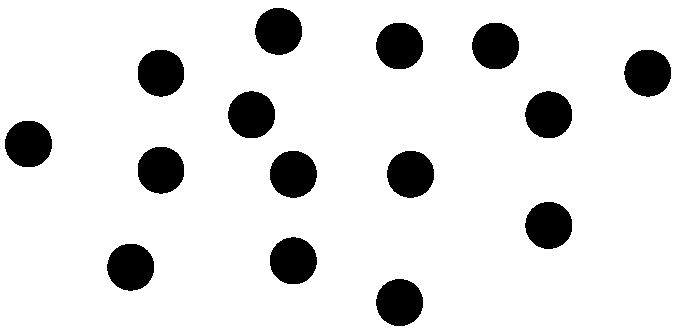
\includegraphics[scale=0.4]{ChugMachine.pdf}
        }
        \hspace{5mm}
        \rule{0.8pt}{4cm}
        \hspace{5mm}
        \subfigure{
            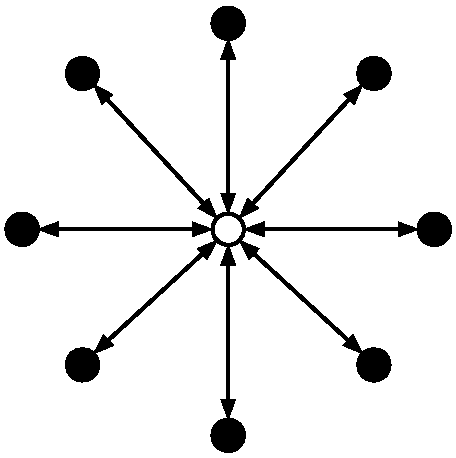
\includegraphics[scale=0.5]{SingleCluster.pdf}
        }
    \end{figure}

    \inote{
        \item What is Process Cooperativity?
        \item White = channel \& black = a process.
        \item Can think of channel a mechanism for passing information between processes. 
            \begin{itemize}
                \item These are nice functional abstractions of things like locks, shared-memory, \etc 
            \end{itemize}
        \item Left: Cloud of processes with no interaction.
        \item Right: We see a definite structure caused by some sharing of information.
              This is the core of recognizing cooperation, namely, recognizing these 
                structures when they exist.
    }
\end{slide}

\begin{slide}
    What does Cooperativity give us?
    \begin{figure} 
    \centering
        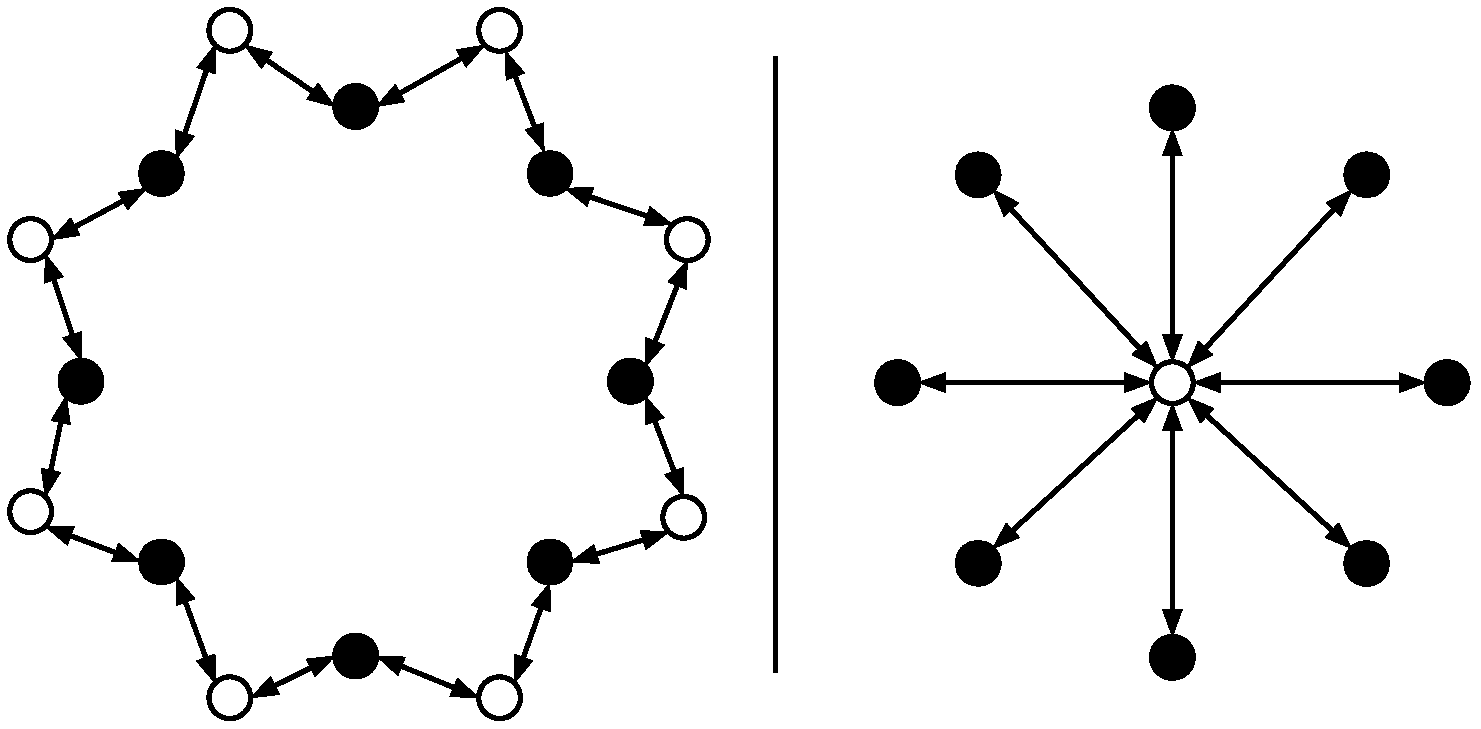
\includegraphics[scale=0.4]{RingVCluster.pdf}
        \label{fig:RingVCluster}
    \end{figure}

    \note{
        What does Cooperativity give us? \hfill
        What's the difference in the behaviour of cooperation in the left/right 
            applications?
        \begin{itemize}
            \item Left: A Ring, 
                \begin{itemize}{\scriptsize
                    \item the level of parallelism is nearly nil. 
                    \item Each process is cooperating yes, but granularity 
                        is very fine.
                    }
                \end{itemize}

            \item Right: A Star, 
                \begin{itemize}{\scriptsize
                    \item the level of parallelism is nearly full. 
                    \item Each process is cooperating,
                        {\bf not reliant on more than one} other process.
                    }
                \end{itemize}
            \item In both, the whole system is communicating, but with 
                cooperation, we can find the level of parallelism possible.
        \end{itemize}
        \hfill
        Next: Knowing this, how can we recognize cooperativity?
        Seems to be all about recording interactions with the channel.
    }
\end{slide}


%%%%%%%%%%%%%%%%%%%%%%%%%%%%%%%%%%%%%%%%%%%%%%%%%%%%%%%%%%%%%%%%%%%%%%%%%%%%%%
\subsection{Message Passing}

\begin{slide}
    We use a Symmetric, Synchronous, Message-Passing Primitive: 
            \begin{center} {\tt\large swap} \end{center}
    \begin{itemize}
        \item Purely captures cooperation of processes through synchronizing on
                a shared channel.
    \end{itemize}
    \inote{
        \item Symmetric, Synchronous, Message-Passing primitive.
        \item Symmetric:
            \begin{itemize}
                \item Only one message passing primitive: SWAP
            \end{itemize}
        \item Synchronous:
            \begin{itemize}
                \item Blocks until it's partner gets there.
            \end{itemize}
        \item Purely captures cooperation: Simple synchronization representation.
        \item This is really what I based the language on. 
        \item So, what does the rest of the language look like.
    }
\end{slide}


